\section{Spécificités de la migration d'UI vers les tables interactives}
\label{sec:chap2:4}
Les tables interactives sont des surfaces qui offrent la possibilité d'interagir avec des systèmes interactifs à travers des UI. Les spécificités d'interactions entre les utilisateurs et ces tables interactives peuvent être décrites avec des interactions instrumentales~\cite{Beaudouin-Lafon2000}. Une interaction instrumentale est une action d'un utilisateur à l'aide de dispositifs physiques (écran tactile par exemple) et de composants graphiques (boutons, scrolls par exemple) pour modifier ou accéder à des objets d'un domaine (images, données numériques, etc.). Ensuite une interaction en sortie est une réponse traduite en une réaction ou un feedback par les instruments d'interaction en sortie. La figure~\ref{fig:chap2:1} montre les différents éléments de ce modèle d'interaction, les instruments servant de moyen d'interactions  pour l'utilisateur sont constitués de l'écran tactile et des composants graphiques. La migration d'une UI décrite suivant un autre modèle d'interactions vers ce modèle implique l'adaptation des objets du domaine et des interactions de l'UI de départ aux nouveaux instruments qui constituent la plateforme d'arrivée. L'adaptation des différents aspects de l'UI de départ à la table interactive, se fait suivant un ensemble de principes et des recommandations liés aux tables interactives, dans l'objectif d'avoir une UI respectant ses critères ergonomiques.


Dans l'objectif d'identifier et de caractériser les principes de conception des UI pour les tables interactives, cette section étudie les différents éléments qui composent le modèle d'interaction d'une table interactive (instruments matériels, instruments logiciels, représentation des interactions  en entrée et en sortie entre les utilisateurs et les objets du domaine). Elle  présente l'ensemble des principes de conception des UI liées aux tables interactives nécessaires pour la migration. 
	
\subsection{Modèle d'interactions d'une table interactive}
Les instruments d'interactions constituent l'ensemble des dispositifs matériels et logiciels d'une table interactive qui permettent d'interagir avec un SI. Les dispositifs matériels d'interactions sont des moyens d'interactions en entrée (actions) ou en sortie (réactions et feedback) cf. figure~\ref{fig:chap2:1}. Et les bibliothèques graphiques sont des instruments logiciels pour décrire des interfaces utilisateurs graphiques dans le cadre des tables interactives. Dans ce paragraphe nous nous appuierons sur des tables interactives (Microsoft PixelSense, TangiSense, DiamondTouch, etc.) pour caractériser les dispositifs matériels et d'interaction, les bibliothèques graphiques et les modalités d'interactions des tables interactives. 

\begin{figure}[ht]
\begin{center}
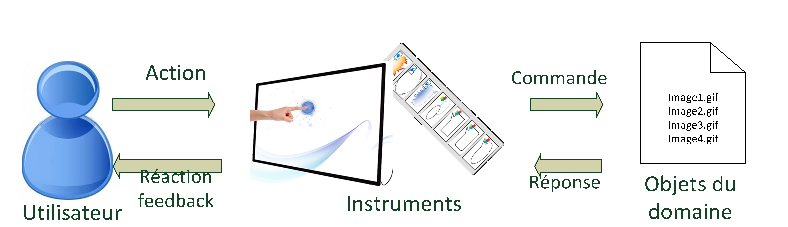
\includegraphics[width=360pt]{chap2/img-1}
\caption[b]{Modèle d'interaction instrumentale d'une table interactive}
\label{fig:chap2:1}
\end{center}
\end{figure}
\subsubsection{Les dispositifs matériels d'interaction d'une table interactive}
\label{sec:chap2:3:1}
Dans ce paragraphe nous étudions les instruments d'interactions de trois tables interactives. Nous étudions d'abord DiamonTouch ~\cite{Dietz2001} qui est l'une des première table interactive utilisée dans un cadre non expérimental, elle fut industrialisée par MERL~\cite{MitsubishiElectricResearchLaboratoriesb}, nous l'étudions car elle comporte une bibliothèque graphique DiamondSpin et permet de décrire des interactions multi utilisateurs, collaboratives et tactiles. Ensuite, l'on s'intéresse à metaDesk ~\cite{Ullmer1997} qui supporte que des objets tangibles comme moyen d'interaction. Enfin nous nous intéresserons aux tables Microsoft PixelSense 1.0 et 2.0 ~\cite{Microsoft2011} pour leurs bibliothèques graphiques et leurs moyens d'interactions, contrairement aux deux autres tables précédentes, les tables Surface supportent à la fois les interactions collaboratives, tangibles et tactiles.

\paragraph {DiamondTouch}-
\label{sec:chap2:3:1:1}
Les moyens d'interaction de la table DiamonTouch sont une surface tactile non capacitif pour les interactions en entrée et un vidéo projecteur pour les interactions en sortie. Cette table supporte des interactions multi utilisateurs et elle est capable d'identifier  les contacts de chaque utilisateus autour de la table. Elle ne supporte pas les interactions tangibles car elle ne peut pas détecter des objets ou des tags. Cette table permet de décrire des UI collaboratives. Les UI collaboratives pour les tables interactives ont pour objectif de permettre à plusieurs utilisateurs de partager en même temps une UI.  Dans le cadre de la  table interactive DiamondTouch les utilisateurs d'une UI collaborative partagent un même espace (la table interactive) et il est possible de créer à chaque utilisateur son espace de travail. Cette solution implique une répartition géographique fixe autour de la table. En effet pour migrer l'UI de l'application CBA par exemple sur une table DiamondTouch, il est indispensable de connaitre le nombre d'utilisateurs de l'UI migrée car chaque utilisateur doit être assis sur une chaise pour utiliser la table(cf. figure~\ref{fig:chap2:17}). DiamondTouch ne permet aux utilisateurs d'être debout pendant l'utilisation de la surface d'affichage.  
 
\begin{figure}[h]
\begin{center}
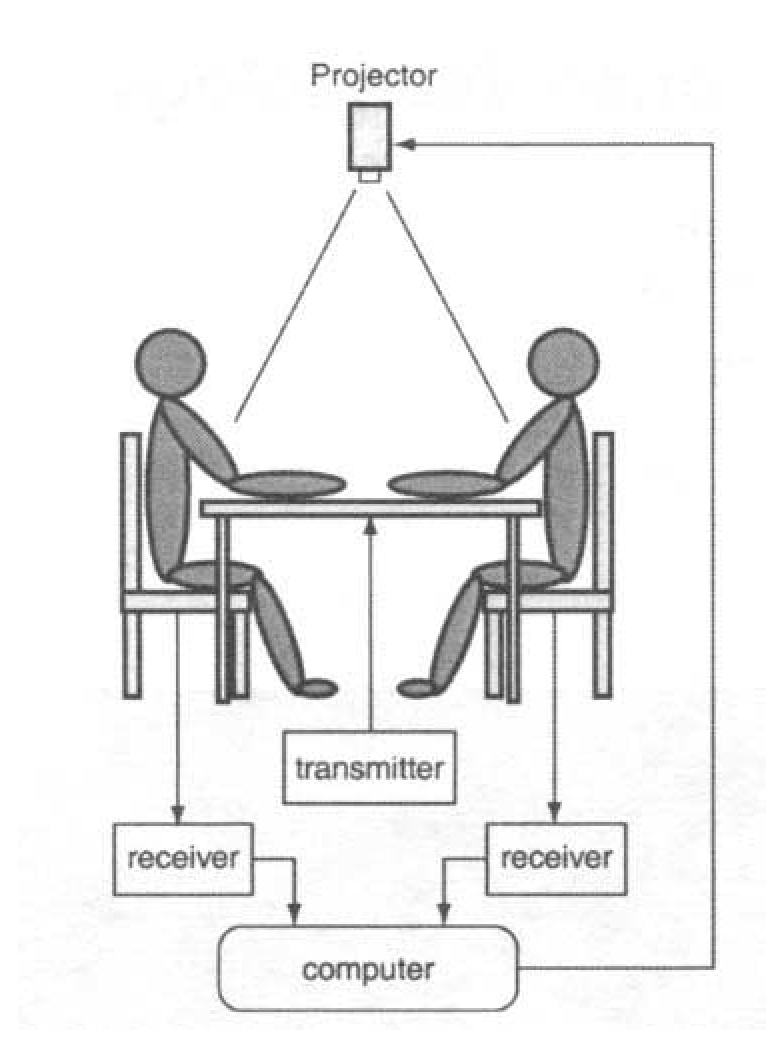
\includegraphics[scale=.4]{chap2/img-10}
\caption{Table interactive DiamondTouch}\label{fig:chap2:10}
\label{fig:chap2:17}
\end{center}
\end{figure}

\paragraph {metaDESK}-
\label{sec:chap2:3:1:2}
Les moyens d'interaction de la table metaDESK sont constitués des objets tangibles et de caméra infrarouge. Ces objets permettent à chaque utilisateur de manipuler des objets virtuels associés aux objets physiques. Elle ne limite pas le nombre d'utilisateurs comme la table DiamondTouch et permet à chaque utilisateur d'être mobile autour de la table. Cette Table permet de décrire des UI tangibles (TUI).

Ulmer et Ishii ~\cite{Ishii1997} définissent un TUI comme des systèmes interactifs qui utilisent des objets physiques pour représenter et utiliser des informations digitales. Le mapping entre le monde physique et digital peut se faire en représentant les différents composants graphiques d'une UI graphique à l'aide des objets concrets. La conception de TUI pour la table metaDESK~\cite{Ishii1997}, les concepteurs associent une lentille à une fenêtre, un plateau à un menu, etc. comme l'indique la figure~\ref{fig:chap2:12} d'instanciation physique des éléments GUI de metaDESK de la figure~\ref{fig:chap2:12}. Ce type d'association permet de concrétiser des composants graphiques virtuels à travers des objets physiques.\\
Dans le cadre de la migration d'une UI desktop vers la table metaDESK, toutes les interactions de l'UI de départ doivent être adaptées ou émulées avec des objets tangibles. En considérant l'UI de l'application CBA par exemple, le formulaire \textit{Ressources} doit être affiché et rempli avec des objets tangibles, la sélection de la taille ou de la police peuvent être émuler avec des objets circulaires en les tournant par exemple. Par ailleurs l'émulation d'un clavier à l'aide d'un objet tangible pour la saisie des textes est possible mais n'est pas facilement utilisable~\cite{MenuTangible}. Les tables interactives uniquement tangibles comme metaDESK ou TangiSense~\cite{Kubicki2009} sont en générale conçues pour faire de la réalité augmentée pour des applications de cartographie par exemple.
\begin{figure}[ht]
\begin{center}
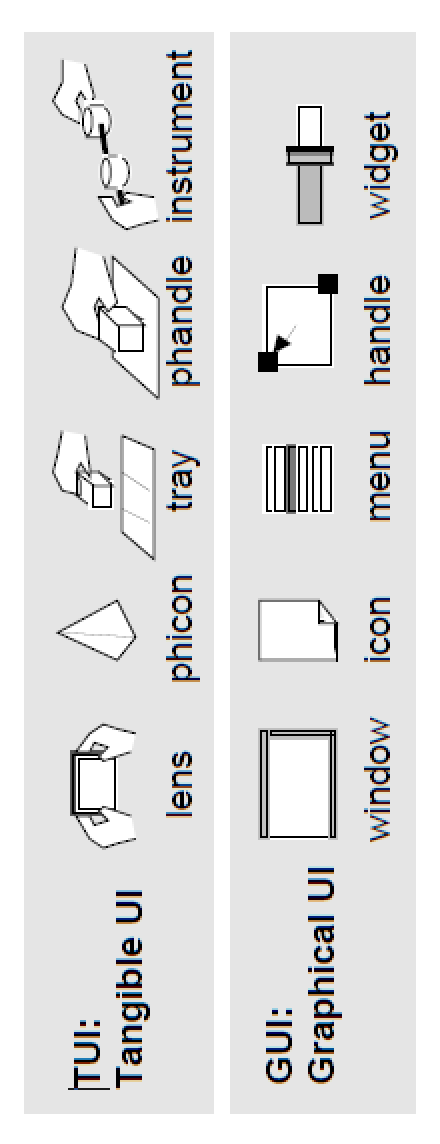
\includegraphics[angle=270,scale=.6]{chap2/img-12}
\caption{Instanciation physique des éléments GUI dans TUI}
\label{fig:chap2:12}
\end{center}
\end{figure}

\paragraph {Microsoft PixelSense }
\label{sec:chap2:3:1:3}
Les moyens d'interaction de la table interactive Microsoft PixelSense sont un écran tactile permettant la reconnaissance des objets physiques, un clavier virtuel et des dispositifs sonores. Elles permettent de décrire des UI tactiles et tangibles par l'utilisation des tags. Elles supportent  50 contacts simultanés et permet donc de décrire des UI multi utilisateurs dans la limite des contacts supportés. En effet une UI ne peut pas supporter plus de 50 points de contacts simultanés, cette contrainte et la taille de l'écran limite le nombre d'utilisateurs utilisant une application sur cette table au même moment.

Cette plateforme permet la description de TUI par la reconnaissance des Tags et la forme des objets. L'utilisation de tags permet de ne pas limiter les objets à utiliser dans la description des UI. Les tags sont des codes barres à deux dimensions qui sont facilement identifiables par la table surface. La Surface offre deux types tags : Identity tags et Byte tags\footnote{Les Identity tags sont des tags sur avec une plage de valeurs sur 128 bits, les Byte tags on une plage de valeurs sur 8 bits}. Ils peuvent être utilisés pour reconnaître des objets physiques ou les distinguer parmi plusieurs, pour déclencher une commande ou une action (afficher un menu ou une application par exemple), pour pointer et orienter une application par un objet tagué peut être utilisé pour le contrôle de volume car il peut détecter le changement d'angle d'un objet.

\paragraph{Résumé}
\label{sec:chap2:3:1:4}
Les tables interactives de manière générale ont deux types de dispositifs physiques d'interactions: les dispositifs d'interaction en entrée qui  peuvent être tactiles et/ou tangibles et les dispositifs d'interaction en sortie qui sont des surfaces d'affichage. Ces surfaces sont de tailles variables et de différentes formes (rectangulaire, circulaire, etc.). Elles peuvent être disposées de manière horizontale (pour DiamondTouch, TangiSense, Microsoft PixelSense 1.0 et 2.0) ou de manière verticale (pour Microsoft PixelSense 2.0, etc. ).
 
Le nombre d'utilisateurs et leurs dispositions autour de la surface d'affichage sont des éléments qui permettent de caractériser les interactions des tables interactives. En effet ces deux caractéristiques impactent la conception des UI car une UI destinée à plusieurs personnes doit permettre l'accessibilité des différentes fonctionnalités à tous les utilisateurs et elle doit aussi prendre en compte le partage des éléments de l'UI (menus, visualisation des contenus, etc.)

\fbox{\parbox{0.9\textwidth}{
Les dispositifs matériels des tables interactives permettent de décrire des UI multi utilisateurs, co-localisées, tactiles et tangibles. La migration des UI des applications qui ne prennent pas en compte ces caractéristiques soulève des problématiques liées à la prise en compte des différents moyens d'interactions en entrée et en sortie des tables interactives, du nombre d'utilisateurs et de la disposition des utilisateurs par rapport à la surface d'affichage.}}

\subsubsection{Bibliothèques graphiques des tables interactives}
\label{sec:chap2:3:2}
Les bibliothèques graphiques sont des boîtes à outils logiciels qui contiennent des éléments pour décrire des UI graphiques; dans le modèle d'interactions des tables interactives, les composants graphiques sont des instruments logiciels qui permettent de faire le lien entre les dispositifs matériels d'interactions et les objets d'un domaine. Elles offrent des composants graphiques adaptés aux moyens d'interactions d'une plateforme spécifique. Dans cette section nous présentons quelques bibliothèques graphiques spécifiques aux tables interactives.

\paragraph{DiamondSpin}
\label{sec:chap2:2:2:1} ~\cite{Shen2004} est une bibliothèque graphique pour table interactive qui offre des composants graphiques adaptés à plusieurs utilisateurs. En effet, elle offre des composants graphiques qui permettent : une manipulation des documents visuels, la manipulation directe des éléments d'UI, la possibilité d'utiliser ses doigts, un stylet ou un clavier comme moyen d'interaction, la rotation des composants graphiques, et la possibilité de créer et de gérer des espaces privés pour chaque utilisateur. Les composants graphiques \textit{DSContainer, DSPanel, DSWindow, DSFrame} (cf. figure \ref{fig:chap2:2}) par exemple permettent d'avoir un container qui regroupe un ensemble de composants graphiques qu'un utilisateur peut déplacer en fonction de sa position. 
\begin{figure}[ht]
\begin{center}
\includegraphics[angle=90, width=258pt]{chap2/img-16}
\caption{Instances des container DiamondSpin}\label{fig:chap2:2}
\end{center}
\end{figure}

\paragraph{Surface SDK  1.0 et 2.0}\label{sec:chap2:2:2:2} ~\cite{Microsoft2012} sont des API et des boîte à outils pour développer des applications pour une Table interactive Microsoft (1.0 et 2.0). Ils font partie du Framework .Net et offrent des bibliothèques graphiques pour concevoir des UI WPF ~\cite{MicrosoftWPF2012} et XNA ~\cite{MicrosoftXNA2012}. Ces bibliothèques graphiques offrent des composants graphiques permettant la reconnaissance des formes d'objets, l'utilisation des tags, 50 points de contacts simultanés, la détection de l'orientation des touches, etc. Ces facilités par rapport à la bibliothèque graphique DiamondSpin évitent au programmeur la gestion du déplacement ou la rotation des composants graphiques par exemple. En effet un \textit{ScatterView} (Figure \ref{fig:chap2:3}) définie le déplacement ou la rotation de manière intrinsèque.
\begin{figure}[ht]
\begin{center}
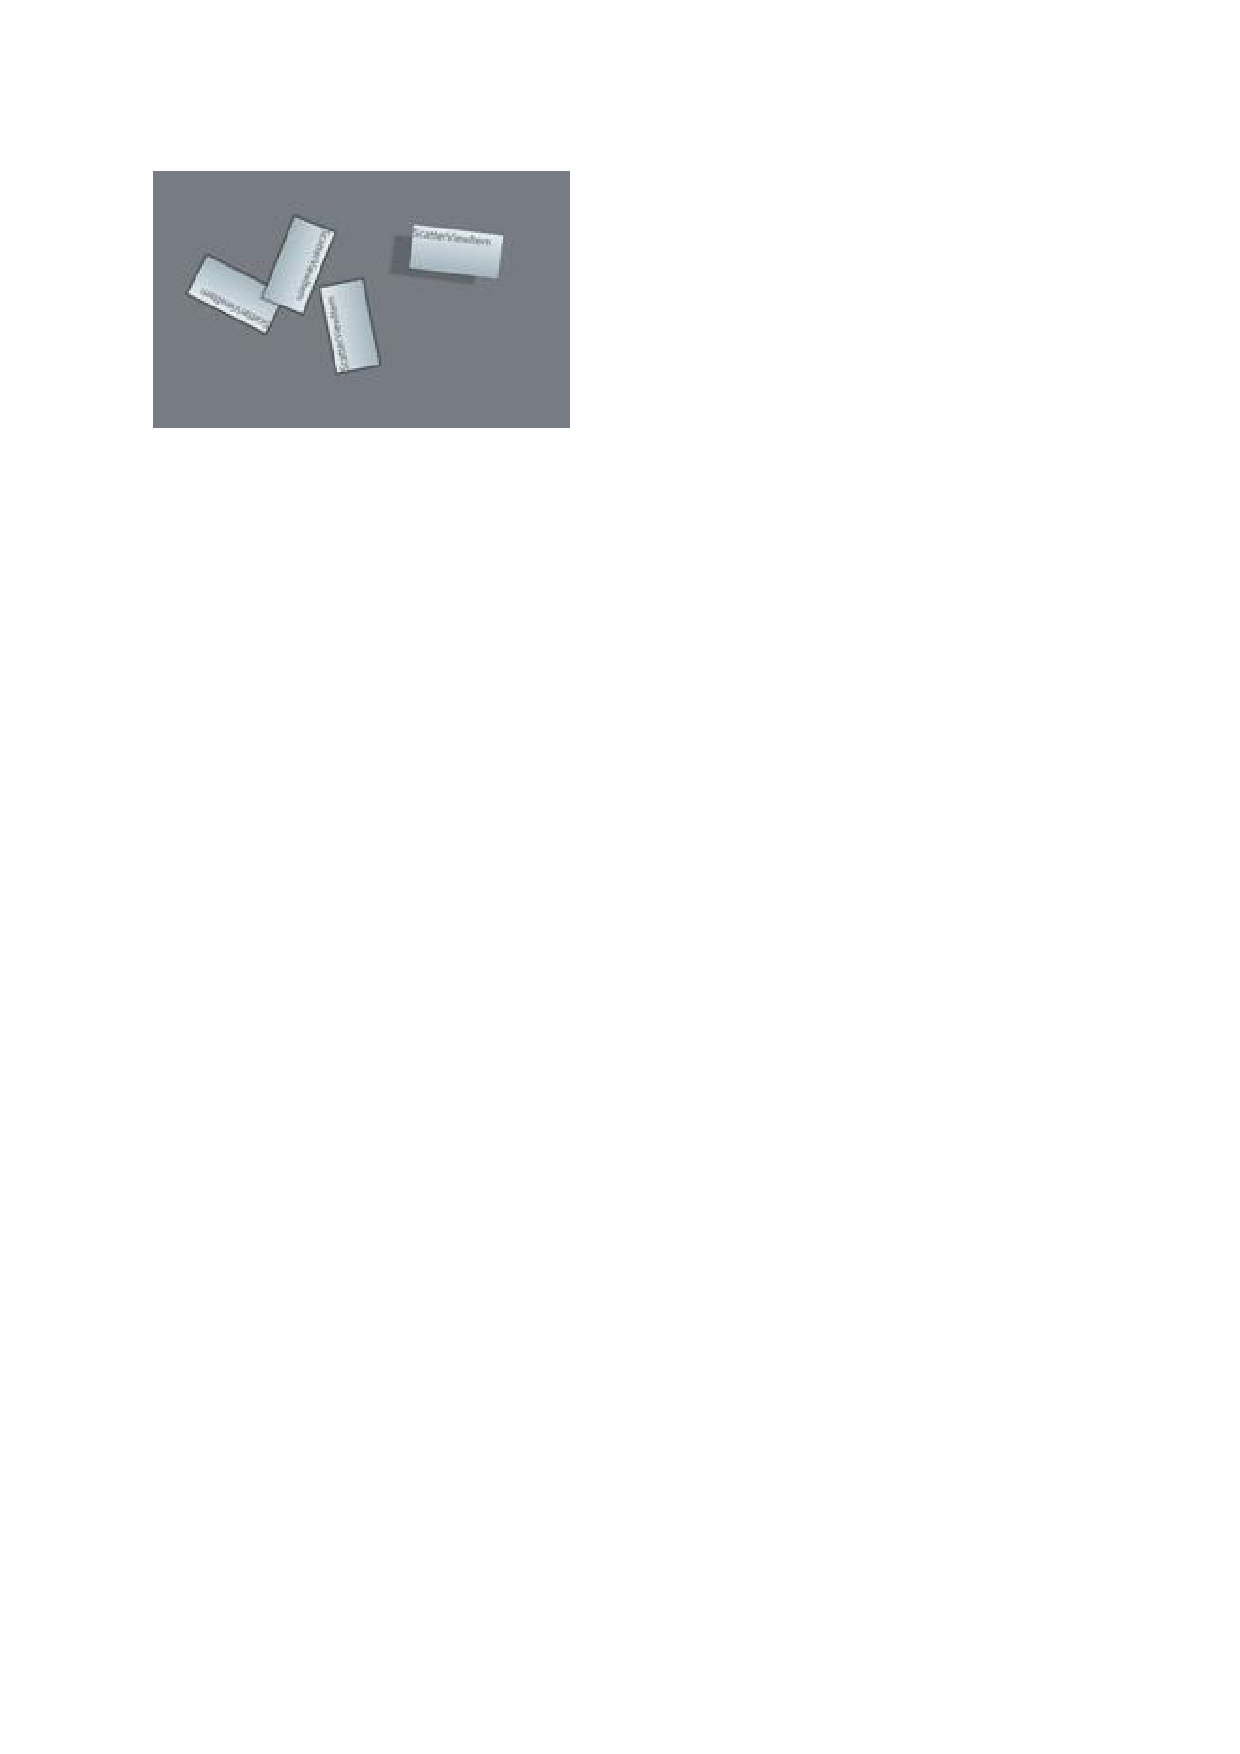
\includegraphics[width=200pt]{chap2/img-4}
\caption{Exemple de ScatterView}
\label{fig:chap2:3}
\end{center}
\end{figure}
\paragraph{Résumé}
\label{sec:chap2:2:2:3}
La bibliothèque DiamondSpin permet d'utiliser la table DiamondTouch à l'instar d'un bureau virtuel par plusieurs personnes assises autour de la table. Elle offre aussi des composants graphiques basés sur la métaphore du papier~\cite{Besacier2007}. La métaphore du papier permet l'utilisation des éléments graphiques d'un container comme une feuille de papier en ayant la possibilité de plier, retourner, dupliquer ou déchirer le container, sur une table interactive cette métaphore permet de conserver les actions qu'on réalise sur une table de travail concrète.\\ 
La bibliothèque Surface SDK permet de décrire des TUI à l'aide des tags. De manière générale, les bibliothèques graphiques des tables interactives offrent des composants graphiques qui ont des interactions (rotation, redimensionnement, déplacement, tags, etc.) adaptées pour la description des UI pour les tables interactives. Elles permettent d'affiner les caractéristiques des tables interactives en précisant si une table interactive supporte ou non des interactions tangibles, si elle a des composants graphiques accessibles par tous les utilisateurs par exemple.\\

\fbox{\parbox{0.9\textwidth}{
Dans le cadre de la migration, le changement de bibliothèque graphique implique une nouvelle conception de l'UI de départ pour rendre accessible ses fonctionnalités sur la plateforme d'arrivée en utilisant les composants graphiques adaptés aux dispositifs physiques de la table interactive.}}

\subsubsection{Modalités d'interactions}
\label{sec:chap2:3:3}
Nigay ~\cite{Nigay1994a} propose une définition de la modalité d'interaction comme un couple <d, l> constitué  d'un dispositif d'interaction et d'un langage d'interaction ~\cite{Nigay1994a}: - d désigne un dispositif physique (par exemple, une souris, une caméra, un écran, un haut-parleur), - l dénote un système représentationnel, c'est-à-dire un système conventionnel structuré de signes assurant une fonction de communication (par exemple, un langage pseudo naturel, un graphe, une table).

\fbox{\parbox{0.9\textwidth}{
La migration des UI vers les tables interactives implique un changement des dispositifs d'interactions et la possibilité de décrire des équivalences entre les modalités d'interactions des plateformes de départ et celles des tables interactives.}}\\

Dans cette section nous abordons la problématique liée aux changements des modalités d'interactions des UI à migrer. En effet comment décrire les interactions de l'UI de départ à l'aide des modalités d'interactions de la plateforme d'arrivée? Pour répondre à cette question nous étudions au paragraphe \ref{sec:chap2:3:1} les problèmes liées aux changements de modalités d'interactions pendant la migration. Et au paragraphe \ref{sec:chap2:3:2} nous présentons quelques modèles d'interactions abstraite qui permet de décrire les interactions indépendamment des modalités d'interactions.

\paragraph{Changement de modalité d'interaction}-
\label{sec:chap2:2:3:1}
Considérons comme plateforme de départ un desktop composé d'un écran comme moyen d'interaction en sortie et d'un clavier et d'une souris comme moyen d'interaction en entrée. 
\begin{itemize}
\item La modalité d'interaction en sortie M1  du  desktop est décrite par l'écran et par le langage de description des UI 2D (L1), M1=<Ecran, L1>. Le langage L1 correspond aux composants graphiques tels que labels, champ de texte, boîte de dialogue, etc. d'une bibliothèque graphique.
\item La modalité d'interaction en entrée M2  du  desktop est décrite par le clavier et par le langage des commandes (L2), M2=<Clavier, L2>. Le langage L2 décrit pour chaque actions les tâches réalisables à l'aide d'un clavier sur une UI graphique, ces actions sont par exemple : copier avec Ctrl+C, couper avec Ctrl+X, coller avec Ctrl+V, saisir un texte avec les touches alphanumériques, valider avec la touche entrée, etc. 
\item La modalité d'interaction en entrée M3  du  desktop est décrite par la souris et par le langage de manipulation directe d'une UI 2D (L3), M3=<Souris, L3>. Le langage L3 décrit les actions réalisables à l'aide d'une souris sur une UI graphique, ces actions sont par exemple : cliquer et valider pour sélectionner un composant graphique, cliquer et déplacer pour sélectionner un texte, déplacer un élément, redimensionner, etc. 
\end{itemize}

Et considérant maintenant que la table interactive cible est composée d'un écran tactile, d'un clavier virtuel et de la reconnaissance des objets physiques comme moyens d'interactions.
\begin{itemize}
\item La modalité d'interaction en sortie M'1  de la table interactive est décrite par l'écran tactile et par le langage de description des UI 2D (L'1), M'1=<Ecran Tactile, L'1>. Le langage L'1 correspond à la bibliothèque graphique de la table interactive qui contient les composants graphiques tels que labels, champ de texte, images, fenêtre, etc.
\item La modalité d'interaction en entrée M'2  de la table interactive est décrite par l'écran tactile et par le langage de manipulation tactile d'une UI 2D (L'2), M'2=< Ecran Tactile, L'2>. Le langage L'2 décrit les actions utilisateurs sur un écran tactile. Ces actions sont par exemple : toucher avec un doigt pour activer ou sélectionner un élément, toucher avec deux doigts et déplacer pour agrandir, réduire, tourner des composants graphiques, etc.
\item La modalité d'interaction en entrée M'3  de la table interactive est décrite par le clavier virtuel  et par le langage de commande  (L'3), M'3=< Ecran Tactile, L'3>. Le langage L'3 décrit les actions utilisateurs réalisables avec un clavier virtuel tel que saisir un texte.
\item La modalité d'interaction en entrée M'4  de la table interactive est décrite par l'écran tactile et par le langage de manipulation des objets tangibles (L'4), M'4=< Objets Tangibles, L'4>. Le langage L'4 décrit les actions utilisateurs sur un écran tactile à l'aide des objets tangibles. Ces actions sont par exemple : poser un objet pour afficher un menu ou un formulaire, déplacer un objet physique pour déplacer l'objet virtuel associé, tourner un objet physique pour sélectionner une fonctionnalité, etc.
\end{itemize}

Les langages d'interaction L1 et L'1 permettent de décrire les interactions en sortie des UI des applications source et cible. Ces langages peuvent être modélisés en se basant sur des boîtes à outils indépendantes des dispositifs d'interactions en sortie. Crease dans ~\cite{December2001} propose une boîte à outils décrivant des widgets multimodales et indépendantes des dispositifs d'interactions en sortie. Les widgets de Crease~\cite{December2001} restent cependant liées aux dispositifs d'interactions en entrée tels que le clavier et la souris.

Les langages d'interaction L2, L3, L'2, L'3 et L'4 quant à eux permettent de décrire et d'interpréter les interactions en entrée des utilisateurs des plateformes de départ et d'arrivées. Ces langages d'interaction permettent d'associer à chaque action de l'utilisateur un comportement ayant un sens dans l'UI de l'application. Les actions utilisateurs telles que cliquer, sélectionner, Ctrl+C, poser un objet, etc. dépendent des dispositifs d'interactions tandis que les comportements de l'UI dépendent du type d'UI et de l'interprétation souhaitée par le concepteur.\\

\paragraph{Équivalences des modalités d'interactions}
La migration de la plateforme desktop vers une table interactive peut être considérée comme un processus de changement de modalités d'interactions. En effet dans le but de réutiliser l'UI d'une application de départ avec les dispositifs d'interactions de la plateforme d'arrivée, il est possible d'établir des équivalences entre les dispositifs d'interaction et les langages d'interactions des plateformes de départ et d'arrivée.\\
Pour décrire les interactions d'une UI de départ à l'aide des dispositifs d'interaction d'une table interactive, l'une des approches à envisager peut être la mise en correspondance des dispositifs d'interactions en établissant des équivalences entre les différentes modalités d'interactions des plateformes source et cible. Ce qui consiste par exemple à décrire des équivalences d'abord entre les modalités d'interactions en sortie  M1 et M'1 et ensuite entre les modalités d'interactions en entrée M2, M3 et M'2, M'3 M'4.\\
L'équivalence entre M1 et M'1 consiste à comparer les deux dispositifs qui sont des écrans qui peuvent afficher des UI graphiques et les langages L1 et L'1 qui ont des composants graphiques appartenant à des bibliothèques graphiques différentes.
L'équivalence entre les modalités d'interactions en entrée n'est possible que si l'on peut comparer les langages L2, L3, L'2, L'3 et L'4. Ces langages sont décrits en fonction des dispositifs d'interaction et aussi en fonction des applications, en effet chaque concepteur peut décrire un langage propre à son application, l'objectif de ces langages étant de faciliter l'interaction entre un dispositif physique (clavier, souris, écran tactile, etc.) et l'UI de l'application.


%\paragraph{Résumé}
%\label{sec:chap2:2:3:3}
%Dans le processus de migration vers une table interactive, le paragraphe~\ref{sec:chap2:2:3:1} indique les différences entre les modalités d'interactions en entrée sont importantes au niveau du nombre de dispositifs physiques et des langages. 


\subsection{Propriétés caractéristiques du modèle d'interactions des tables interactives }
\label{sec:chap2:3:4}
Les éléments du modèle d'interactions instrumentales des tables interactives tels que les dispositifs matériels d'interactions en entrée et en sortie, les bibliothèques graphiques ou les modalités d'interactions nous permettent d'identifier des propriétés caractéristiques des tables interactives qui impactent la conception des UI pour des tables interactives. 
\subsubsection{Dispositifs d'interactions en entrée }
\label{sec:chap2:3:4:1}
Ces dispositifs influencent la conception des interactions. Dans le cadre des tables interactives nous identifions deux propriétés qui correspondent aux moyens d'interactions tangibles et tactiles.

\fbox{\parbox{0.9\textwidth}{
\begin{prop}{Tangibilité des interactions}\label{prop:chap2:1}\end{prop}
Les dispositifs d'interactions en entrée permettent d'associer des objets physiques aux fonctionnalités\footnote{les objets physiques peuvent être utilisés pour activer des fonctionnalités} ou aux composants graphiques\footnote{les objets physiques peuvent aussi être utilisés pour afficher ou déplacer des objets virtuels} d'une UI.
}}

\fbox{\parbox{0.9\textwidth}{
\begin{prop}{Tactibilité des interactions}\label{prop:chap2:2}\end{prop}
Les dispositifs d'interactions en entrée des tables interactives permettent de décrire des manipulations directes des UI telles que la sélection, l'édition, le redimensionnement, le déplacement, etc. }}

\subsubsection{Dispositifs d'interactions en sortie }
\label{sec:chap2:3:4:2}
Ce sont les surfaces d'affichage des tables interactives, les propriétés caractéristiques liées à la taille et à la disposition des tables interactives qui impactent la conception des UI.\\

\fbox{\parbox{0.9\textwidth}{
\begin{prop}{Taille de la surface d'affichage}\label{prop:chap2:3}\end{prop}
Cette propriété permet d'adapter la taille des composants graphiques par rapport à la taille de l'écran pour faciliter l'utilisation de l'UI.
}}\\

\fbox{\parbox{0.9\textwidth}{
	\begin{prop}{Disposition de la surface d'affichage}\label{prop:chap2:4}\end{prop}
	La surface d'affichage peut être disposée de manière horizontale comme une table de travail ou de manière verticale comme un tableau collaboratif. Ces dispositions influencent l'orientation et l'utilisation des composants graphiques d'une UI.
}}
\subsubsection{Utilisateurs des tables interactives }
\label{sec:chap2:3:4:3}
Les utilisateurs influencent la conception de l'UI par leur nombre et leur répartition autour de la surface d'affichage.\\

\fbox{\parbox{0.9\textwidth}{
	\begin{prop}{Nombre d'utilisateurs}\label{prop:chap2:5}\end{prop}
	Cette propriété permet de savoir comment disposer les éléments de l'UI pour faciliter l'accessibilité en fonction du nombre d'utilisateurs.
}}
\\

\fbox{\parbox{0.9\textwidth}{
	\begin{prop}{Répartition des utilisateurs }\label{prop:chap2:6}\end{prop}
	Cette propriété permet de savoir comment décrire la collaboration entre les utilisateurs autour de la table.
	La répartition de l'espace de travail de chaque utilisateur peut se faire par une division géographique de la surface ou permettre aux utilisateurs d'accéder à toute la surface. 
}}
\subsection{Principes de conception d'UI pour les tables interactives}
\label{sec:chap2:3:5}
Le paragraphe \ref{sec:chap2:3:3} nous montre les différences de modalités d'interactions entre un desktop et une table interactive. Ces différences impactent aussi la conception d'UI pour ces deux plateformes. Besacier et \textit{al.} montrent que la réutilisation des applications desktop sur les tables interactives en adaptant les éléments de l'UI aux métaphores du papier par exemple facilite l'utilisation des UI ~\cite{Besacier2007}. Par ailleurs, une réutilisation d'une application desktop sur des tables interactives sans prise en compte de ses spécificités pose deux problématiques majeures: la transformation de l'UI de départ en UI collaborative d'une part et la transformation d'une GUI en TUI d'autre part. Ces deux caractéristiques font parties de l'ensemble des principes qui guident la conception des UI pour les tables interactives.\\

\fbox{\parbox{0.9\textwidth}{ Les principes de conception d'UI pour une plateforme constituent un ensemble de recommandations pour les concepteurs d'UI qui indiquent comment décrire les aspects tels que les interactions instrumentales, le layout (ou le placement des éléments graphiques), les activités d'une UI et aussi les styles de présentations (couleurs, polices, tailles, etc).}}

Les principes de conceptions sont des recommandations de haut niveau qui doivent être traduites en règles formelles utilisables pendant la migration~\cite{Vanderdonckt1997}.

Dans cette section nous caractérisons les principes de conception pour la migration des UI vers les tables interactives en trois catégories: les principes de conception pour les UI tangibles, les principes de conception pour les UI collaboratives et colocalisées et enfin les autres principes de conception d'UI sur une grande surface d'affichage telles que la taille et la position de la surface d'affichage, l'utilisation en 360 degré de l'UI et le style de l'UI.

\subsubsection{Corpus des principes de conception d'UI pour Microsoft PixelSense}
\label{sec:chap2:3:5:1}
Les principes de conception d'UI pour une Microsoft PixelSense sont décrits sous forme de guidelines (ou recommandations) dans le document \textit{User Experience Design Guideline}~\cite{Microsoft2011}. Ces guidelines sont le fruit des expériences des utilisateurs ayant développé des UI pour cette plateforme. L'objectif de ces guidelines est de faciliter la conception des interfaces utilisateurs naturelles~\cite{Steinberg2012} et intuitives. Ces guidelines couvrent plusieurs aspects du processus de conception des UI tels que la conception des interactions entre les UI et les utilisateurs finaux, les guides de styles pour une cohérence visuelle, les guides d'utilisation des textes, etc. 

\subsubsection{Guidelines pour TUI}
\label{sec:chap2:3:5:2}
Cette catégorie regroupe les recommandations qui permettent de décrire le comportement des éléments de l'UI qui sont des objets virtuels d'une part et l'association entre ces objets virtuels et les objets tangibles d'autre part. L'association peut se faire par des tags qui permettent de marquer les objets physiques ou en se basant sur la forme des objets physiques. Les guidelines de cette catégorie sont inspirées par la propriété~\ref{prop:chap2:1} de tangibilité des interactions.


\shadowbox{\parbox{0.8\textwidth}{
\begin{guide}\label{guide:1}Comportement des objets virtuels\end{guide}
Les comportements des éléments d'une TUI pendant leurs utilisations doivent correspondre aux objets physiques. Les éléments (ou objets virtuels) de l'UI  à migrer doivent être associés à des objets physiques dans le but d'afficher des  menus, des formulaires ou des fenêtres et aussi dans le but d'activer ou d'utiliser des fonctionnalités. 
}}
%\\


\shadowbox{\parbox{0.8\textwidth}{
\begin{guide}\label{guide:2}Objets physiques tagués\end{guide} 
Un tag est associé à un objet virtuel d'une TUI (les objets virtuels sont identifiés grâce à la guideline~\ref{guide:1}). Le déplacement, l'orientation et la position du tag sur l'écran peuvent être associés à des interactions en entrée ou à des comportements de l'objet virtuel associé. 
}}\\


\shadowbox{\parbox{0.8\textwidth}{
\begin{guide}\label{guide:3}Forme des objets physiques\end{guide}
La forme d'un objet physique peut être associé à un objet virtuel ou à une fonctionnalité. Le déplacement, l'orientation et la position d'un objet physique sur l'écran peuvent être associés à des interactions en entrée ou à des comportements de l'objet virtuel associé. L'utilisation de la forme des objets physiques comme moyen d'interaction en entrée nécessite un module de reconnaissance de la forme d'un objet tangible. 
}}\\

En considérant l'UI de l'application CBA à la figure~\ref{fig:chap2:6}, le menu principal et le formulaire \textit{Ressources} par exemple peuvent être associés à un objet physique pour les afficher facilement sur l'écran. Les règles formelles issues de la guideline~\ref{guide:1} permettront d'identifier et de transformer les éléments concrets de l'UI \\ Les tags permettent par exemple d'utiliser deux objets de la forme avec des couleurs différentes et marqués  des deux différents tags pour afficher un menu ou un formulaire. 

\subsubsection{Guidelines pour UI collaborative}
\label{sec:chap2:3:5:3}
Cette catégorie regroupe les recommandations pour la conception d'une UI collaborative et colocalisée pour une table interactive. Les guidelines sont liées à la propriété~\ref{prop:chap2:5} caractérisant le nombre d'utilisateurs et à la propriété~\ref{prop:chap2:6} qui caractérise leur répartition autour de la surface d'affichage. Elles sont aussi liées à la propriété~\ref{prop:chap2:3} et à la propriété~\ref{prop:chap2:4} qui caractérise la taille et la disposition (horizontale ou verticale) de la surface d'affichage des tables interactives. 

\shadowbox{\parbox{0.8\textwidth}{
\begin{guide}\label{guide:4}Nombre d'utilisateurs de l'UI migrée\end{guide}
Cette guideline préconise de prendre en compte le nombre d'utilisateurs de l'UI après la migration. Les UI d'une table interactive peuvent être collaboratives (plusieurs utilisateurs) ou non (dans le cas d'un seul utilisateur). Elle impacte  le couplage entre les tâches et les utilisateurs (qui est spécifié par la guideline~\ref{guide:5}), l'organisation de la surface de travail (qui est spécifiée par la  guideline~\ref{guide:6}) et l'accessibilité des éléments d'une UI collaborative (qui est spécifiée par la guideline~\ref{guide:7}).}}


\shadowbox{\parbox{0.8\textwidth}{
\begin{guide}\label{guide:5}Couplage tâches et utilisateurs d'une UI\end{guide}
Elle est une spécification de la guideline~\ref{guide:4}, car elle préconise dans le cas d'une UI multi utilisateurs :
\begin{itemize}
 \item d'éliminer toute les boîtes de dialogues bloquantes pour les autres utilisateurs de l'UI.
 \item de dupliquer certains éléments de l'UI pour permettre à tous les utilisateurs d'accéder aux éléments de l'UI.
\end{itemize}}}


\shadowbox{\parbox{0.8\textwidth}{
\begin{guide}\label{guide:6}Partage de l'espace de travail\end{guide}
Cette guideline spécifie la guideline~\ref{guide:4} en préconisant des composants graphiques qui facilitent le partage de l'écran dans le cas d'une UI multi utilisateurs.
L'espace de travail doit:
\begin{itemize}
\item permettre à une personne d'utiliser une UI sans avoir l'aide d'autres utilisateurs,
\item permettre à un utilisateur d'utiliser l'UI sans interrompre les utilisateurs présents.
\end{itemize}
 }}
 
 
Le partage de l'espace de travail est implémenté de diverses manières en fonction des tables interactives. La table DiamondTouch~\cite{Dietz2001} par exemple permet aux concepteurs d'associer un utilisateur à une zone de l'écran. Cependant la table Microsoft PixelSense quant à elle ne permet pas une division de l'écran en zones associées aux utilisateurs ou à des fonctionnalités. La figure~\ref{fig:chap2:14} illustre une division de l'écran en quatre zones, ce type de partage d'écran n'est pas autorisé par les guidelines de la table Surface. Dans le cadre de la migration d'UI vers les tables interactives, nous pensons que la division de l'écran en plusieurs zones ne permet pas de décrire des UI collaboratives si elle ne permet pas d'échanges entre les utilisateurs et leur mobilité autour de l'écran.
\begin{figure}[h]
\begin{center}
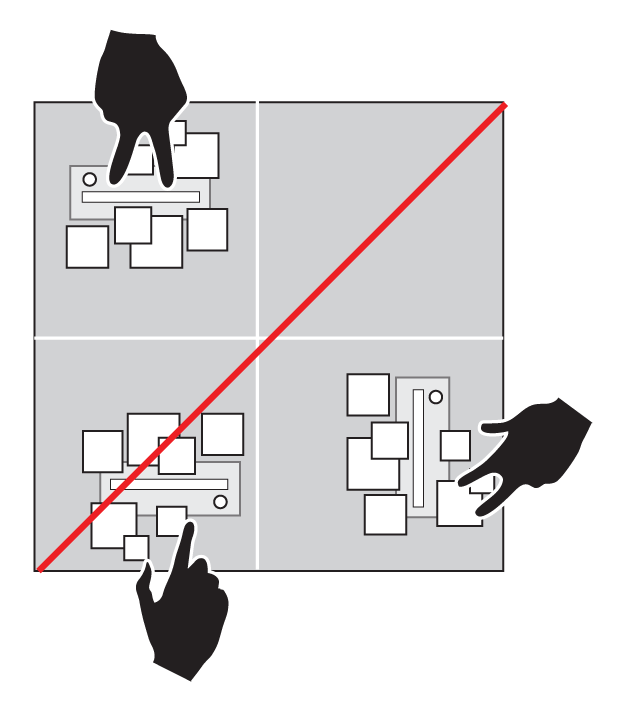
\includegraphics[angle=270,scale=.2]{chap2/img-22} 
\caption{Illustration de partage d'espace entre plusieurs utilisateurs}
\label{fig:chap2:14}
\end{center}
\end{figure}


\shadowbox{\parbox{0.8\textwidth}{
\begin{guide}\label{guide:7}Utilisation 360 degré de l'UI\end{guide}
Cette guideline permet de spécifier la guideline~\ref{guide:4} car elle préconise la sélection des composants graphiques pouvant être utilisés partout autour de la table. Elle rend accessible les éléments d'une UI migrée et renforce la collaboration entre les utilisateurs.}}
\\


La figure \ref{fig:chap2:13} illustre à un cas d'utilisation des composants graphiques utilisables à 360°. 
\begin{figure}[h]
\begin{center}
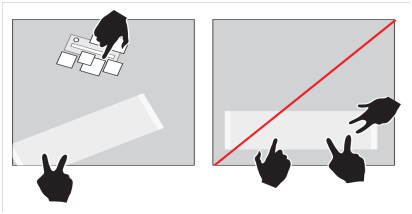
\includegraphics[angle=270,scale=.4]{chap2/img-13} 
\caption{Illustration de la propriété 360°}
\label{fig:chap2:13}
\end{center}
\end{figure}

En considérant que l'UI de l'application CBA (cf. figure~\ref{fig:chap2:6}) est migrée vers une table Surface pour quatre dessinateurs de BD par exemple. Les ressources (images, ballons, etc.) utilisés pour la conception des BD doivent être accessibles par les quatre utilisateurs. La guideline~\ref{guide:6} préconisant le partage de l'espace de travail et la guideline~\ref{guide:6} préconisant l'utilisation des objets 360 degré permettent de décrire une UI sans layout avec des groupes d'éléments utilisables à 360°. La guideline~\ref{guide:5} par exemple permettra de supprimer les composants graphiques bloquants tels que les boites de dialogues de l'UI de l'application CBA.

\subsubsection{Autres guidelines pour les UI sur surface}
\label{sec:chap2:3:5:4}
Les deux catégories de guidelines présentées ci-dessus qui permettent de décrire des UI tangibles et des UI collaboratives (cf. section~\ref{sec:chap2:3:5:3}) ne constituent pas le corpus des guidelines applicables pendant la migration d'une UI vers une table interactive. En effet les apects de l'UI liés au style des composants graphiques, des textes  de l'UI et les aspects liés aux interactions tactiles ne sont pas pris en compte par ces deux catégories de guidelines. 
Cette troisième catégorie regroupe les guidelines de mise en {\oe}uvre des interactions tactiles et des styles de l'UI.
\paragraph{Guidelines pour les interactions tactiles}-
Les tables interactives permettent en général de décrire des interactions tactiles. L'ensemble des actions tactiles de l'utilisateur sont interprétées par le dispositif d'interaction en entrée. Dans le cadre des UI tactiles, il existe des actions tactiles standards pour des interactions de redimensionnement, de déplacement ou de rotation. Par exemple les guidelines des interactions tactiles pour une table Surface~\cite{Microsoft2011} identifient l'ensemble des gestes recommandés aux concepteurs pour la sélection, l'activation, le déplacement, la rotation, le zoom, etc. Cette catégorie de guidelines est liée à la propriété~\ref{prop:chap2:2} de tactibilité des interactions d'une table interactive.

\fbox{\parbox{0.9\textwidth}{
Dans le cadre de la migration de l'UI de l'application CBA  vers les tables interactives Surface, il est indispensable de pouvoir décrire des correspondances entre les interactions tactiles et les interactions du clavier et de la souris de l'UI départ.
}}

\paragraph{Guidelines pour le styles } - 
Cette sous catégorie regroupe l'ensemble des recommandations pour la personnalisation des aspects visuels d'une UI pour une table interactive. 
Ces guidelines peuvent être utilisées dans le cadre d'une migration faisant intervenir les concepteurs comme des exemples pour les inspirer du choix de la forme, des couleurs, des icons et aussi de la diposition des textes d'une UI.
Dans le cas du scénario de migration, le formulaire \textit{Ressources} par exemple peut être migré suivant comme l'indique le tableau~\ref{tab:chap2:1}. 

\begin{table}[h]
\begin{center}
\vspace{3pt} \noindent
\begin{tabular}{|p{143pt}|p{271pt}|}
\hline
Formulaire de l'application de d\'{e}part& Formulaire migré en prenant en compte les guidelines de styles\\ 
\hline
\parbox{143pt}{ 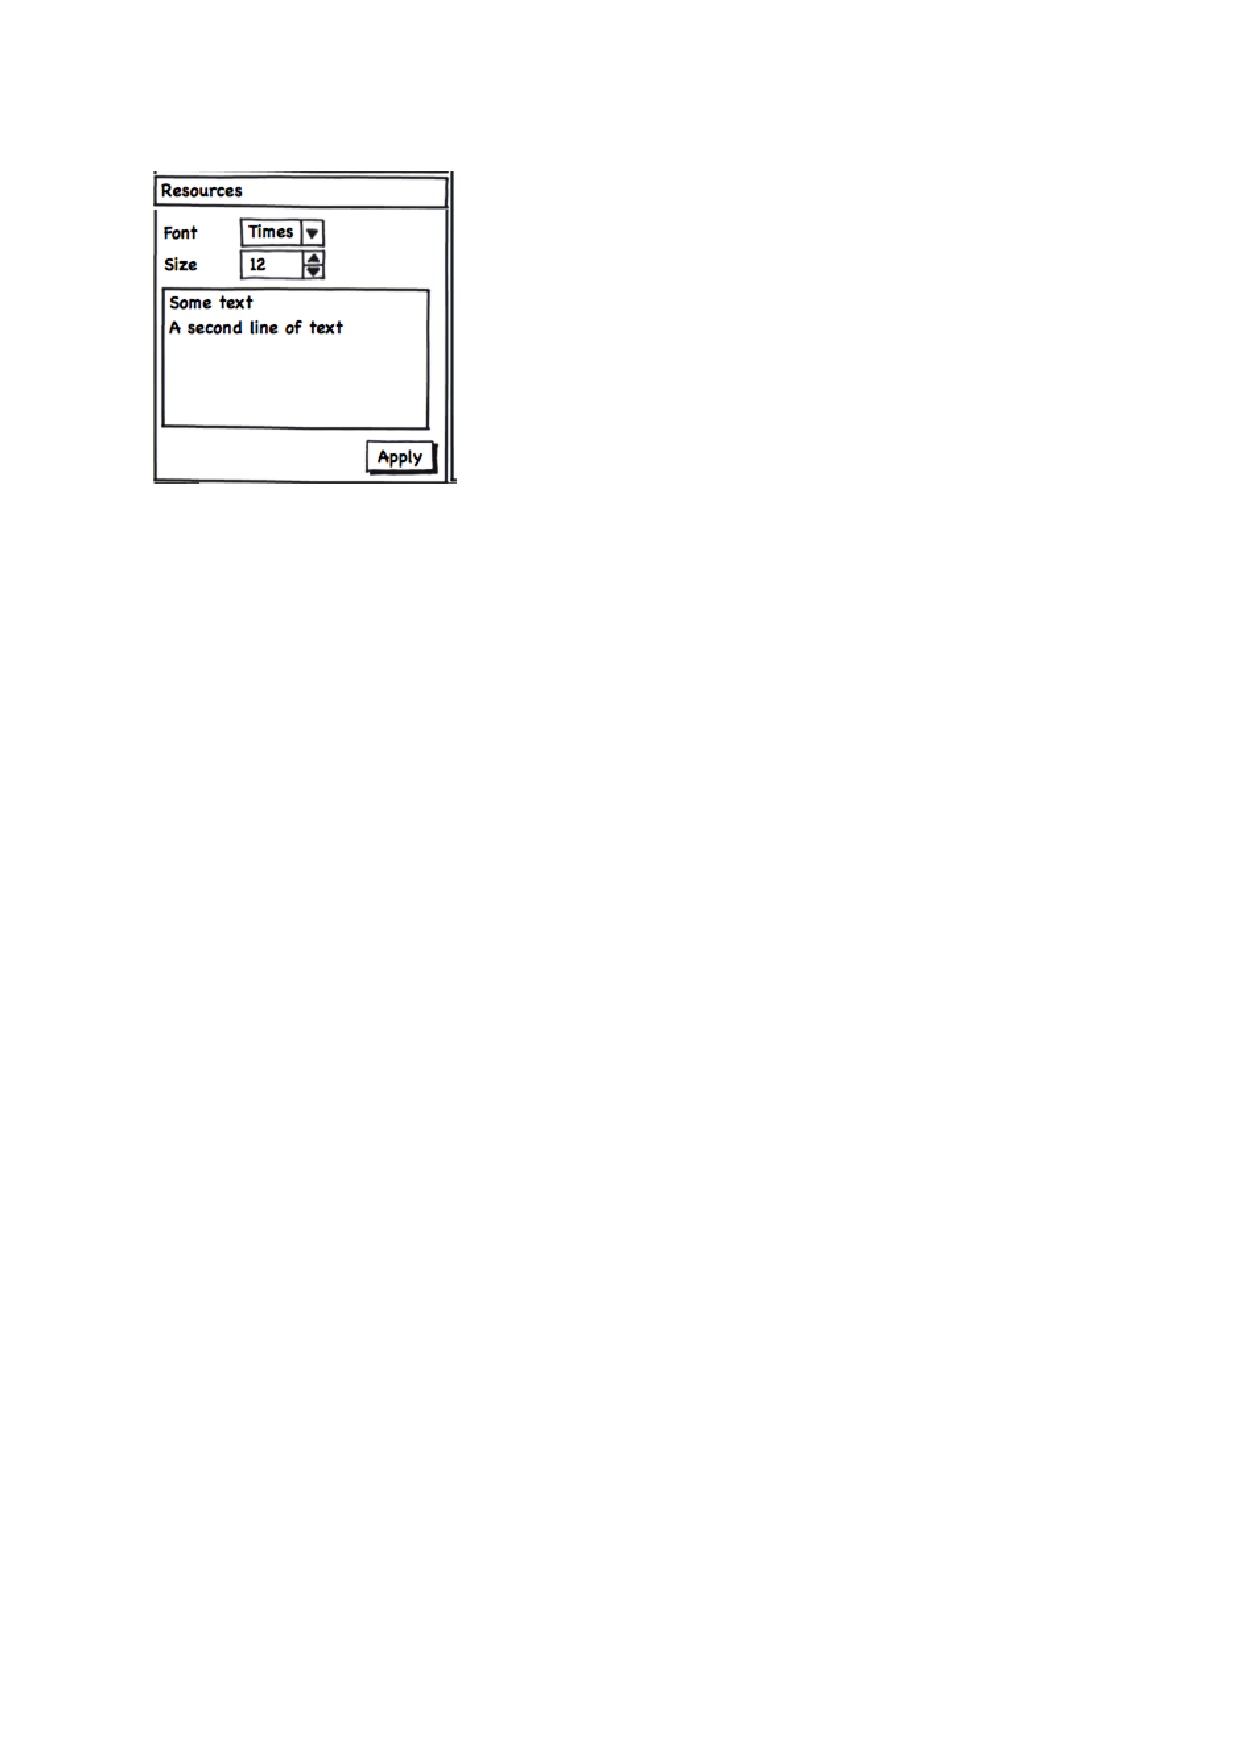
\includegraphics[scale=.8]{chap1/img-12}}& \parbox{271pt}{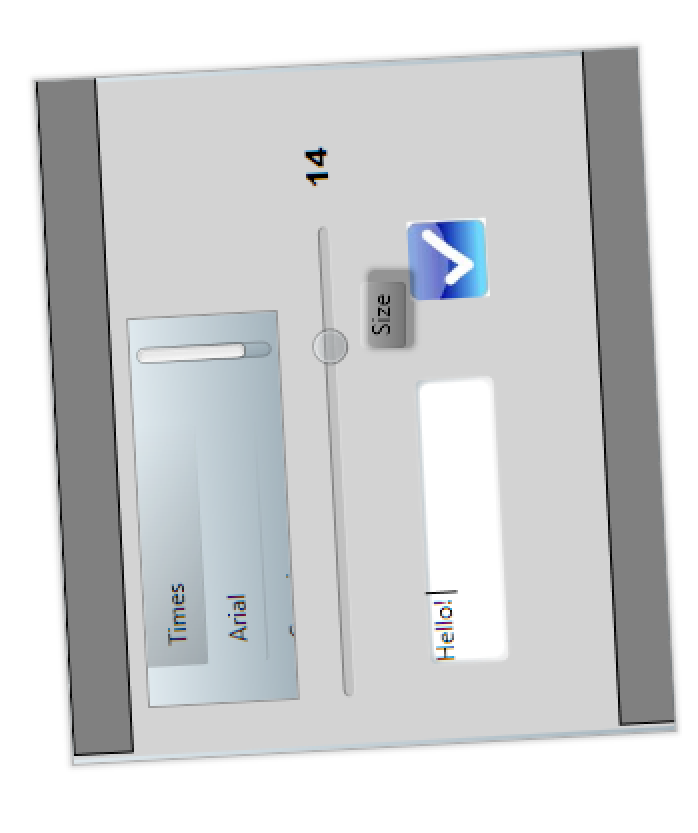
\includegraphics[angle=270, scale=.5]{chap1/img-13}}\\
\hline
\end{tabular}
\vspace{3pt}
\caption{Migration de l'aspect visuel d'un formulaire}
\label{tab:chap2:1}
\end{center}
\end{table}


\subsubsection{Synthèse des guidelines pour la migration d'UI vers les tables interactives}
\label{sec:chap2:3:5:5}
Le corpus de guidelines décrit dans la section~\ref{sec:chap2:3:5} sont des recommandations de haut niveau utiles et nécessaires pour la migration des UI vers une table interactive. Cette caractérisation de ce corpus a pour but de rendre une UI de départ tangible et collaborative pendant la migration tout en considérant les autres modes d'interactions des tables interactives et les aspects visuels de l'UI.

Les liens entre ces guidelines peuvent être synthétisés à l'aide du diagramme de la figure~\ref{fig:chap2:21} qui présente les trois catégories de guidelines, les 7 guidelines pour les UI tangibles et collaboratives et les liens entre ces guidelines. Dans la catégorie des guidelines pour TUI, les guidelines G2 (Objets physiques tagués) et G3 (Forme des objets Physiques) spécifient les moyens d'interactions tangibles à choisir et à associer aux objets virtuels identifiés par la guideline G1. 

Dans la catégorie des guidelines pour UI collaborative, la guideline nombre d'utilisateurs (G4) est spécifiée pour les apects liés aux tâches par la guidelines de couplage des tâches et utilisateurs (G5), la guideline spécifiant le partage de l'espace de travail (G6) entre les utilisateurs et la guideline préconisant l'utilisation 360° de l'UI (G7) permet l'accessibilité de l'UI pour tous les utilisateurs autour de la table.

Dans la catégorie comportant les autres guidelines pour les UI sur surface nous regroupons deux sous catégories; la première concerne les interactions tactiles et la seconde le style de l'UI migrée.
\begin{figure}[h]
\begin{center}
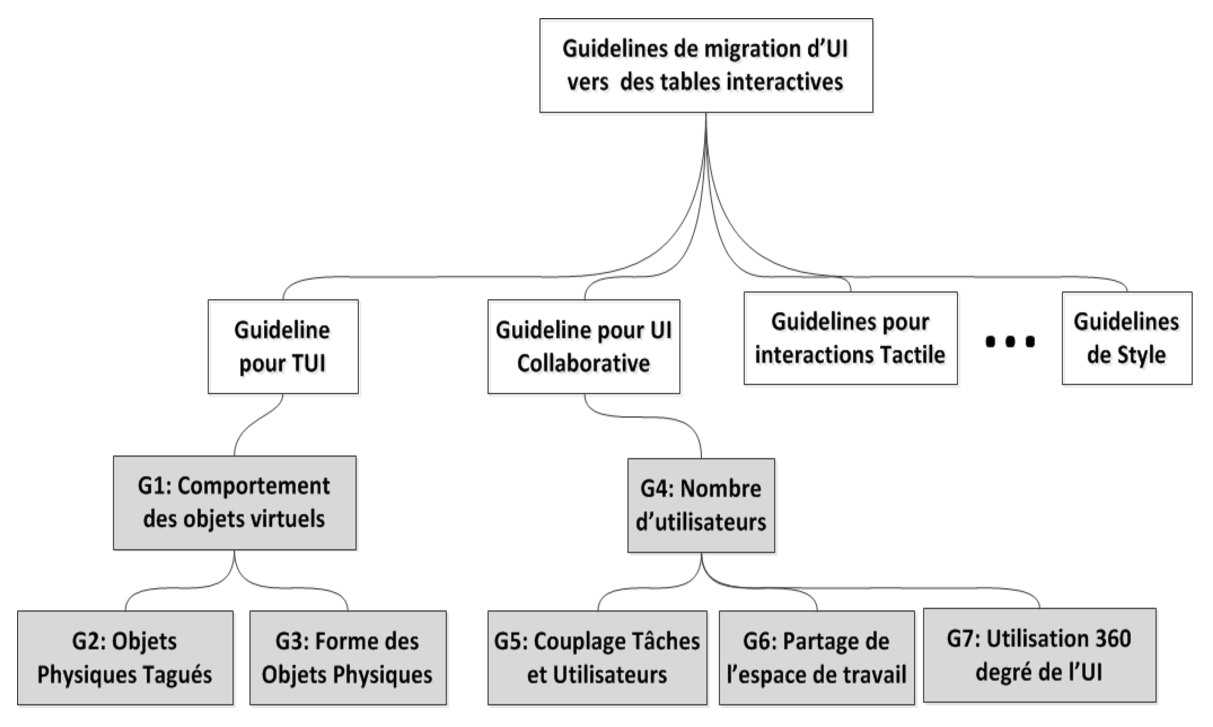
\includegraphics[angle=270, width=450pt]{chap2/img-23-1}
\caption{Liens entre les guidelines de migration d'une UI vers les tables interactives}
\label{fig:chap2:21}
\end{center}
\end{figure}

\section{Concepts pour la migration d'UI}
\label{sec:chap2:5}
Dans les sections précédentes, nous avons identifié quels sont les problèmes liés à la migration d'UI vers une table interactives en partant d'un exemple d'application (à la section~\ref{sec:chap2:2}). Ensuite nous avons aussi identifié les spécificités des tables interactives qui sont importantes pour la migration des UI à travers ses propriétés caractéristiques et les guidelines. Dans cette section nous abordons les problématiques liées aux architectures des applications à migrer et les modèles d'interactions abstraites pour décrire des équivalences entre les modalités d'interactions.

\subsection{Architecture des applications à migrer}
\label{sec:chpa2:4:1}
Les applications à migrer sont des systèmes interactifs (SI) conçus en respectant un modèle d'architecture. Les modèles d'architectures sont des patrons de conception logiciel, ils  préconisent des stratégies de répartition des services qui se traduisent par un ensemble de constituants logiciels. En général, la décomposition minimale des SI préconise une séparation entre le Noyau Fonctionnel (NF) et ceux de l'UI. Dans cette section nous présentons deux modèles d'architectures, d'abord le modèle ARCH~\cite{UIMS1992} qui se base sur des composants logiciels spécifiques et indépendants des plateformes, ensuite le modèle MVC~\cite{Krasner1988} .

\subsubsection{ARCH}
ARCH~\cite{UIMS1992} est un modèle d'architecture qui se base sur des composants conceptuels du modèle de Seeheim~\cite{Pfaff1985}. Comme l'indique la figure~\ref{fig:chap2:5}, ce modèle permet une séparation entre le NF, le Contrôleur de Dialogue (CD) et la Présentation. Les deux pieds de l'arche sont des composants spécifiques à une plateforme; le composant NF décrit un domaine précis et les composants d'Interaction sont liés à des dispositifs du monde réel. Le CD gère l'enchainement des tâches ainsi que les liens avec les objets des deux composants voisins. L'Adaptateur de domaine joue un rôle d'interface avec le composant NF pour corriger les différences de conceptions. Le composant Présentation est une boîte à outils virtuelle, telle que XVT~\cite{Valdes1989} qui implémente les objets de présentations concrétisés finalement par les objets d'interaction de la bibliothèques graphique. 
%PAC-Amodeus~\cite{Nigay1994} est un modèle d'architecture basé sur ARCH, il permet de définir plusieurs contrôleurs de dialogue pour une application grâce aux agents  PAC.  
\begin{figure}[h]
\begin{center}
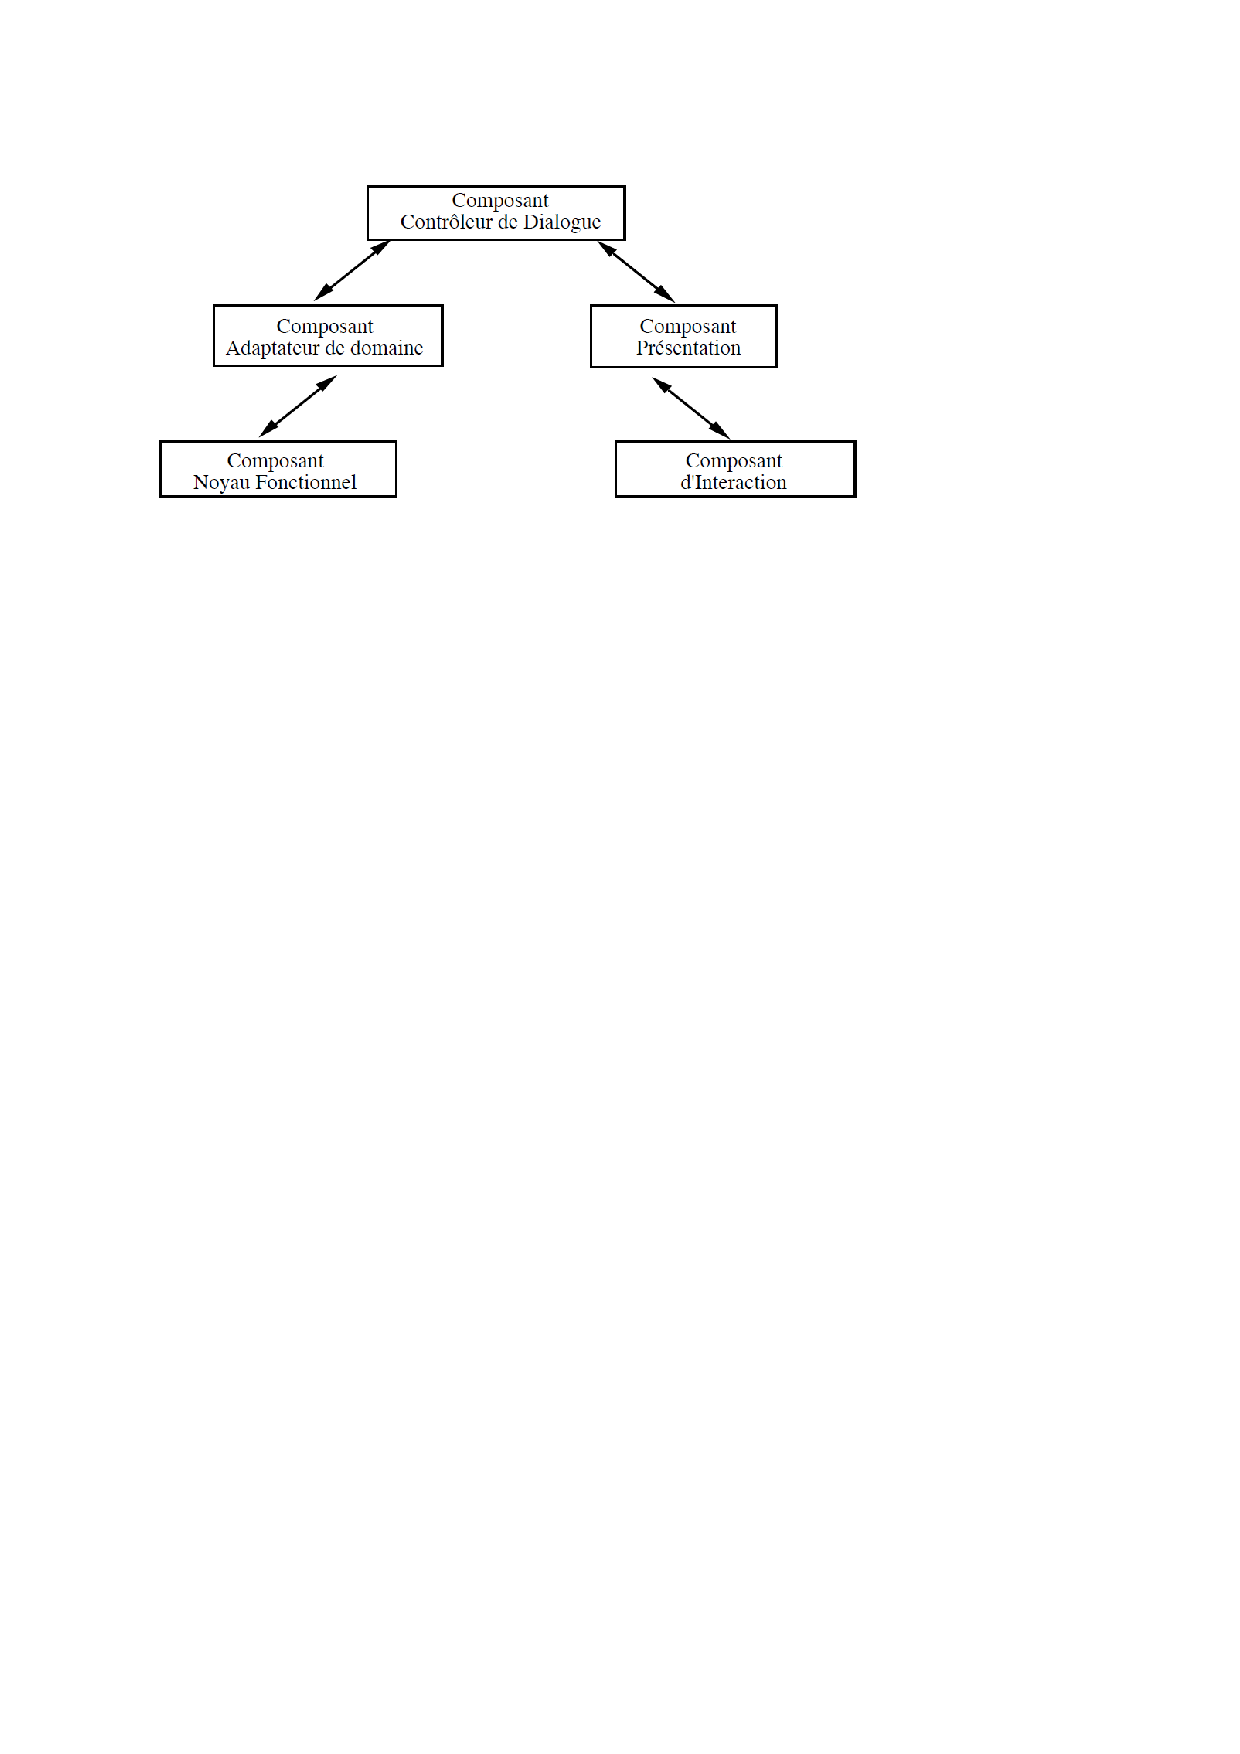
\includegraphics[width=340pt]{chap2/img-7}
\caption{Composants du modèle ARCH}\label{fig:chap2:5}
\end{center}
\end{figure}

\paragraph{Migration d'une application respectant une architecture ARCH}-
Thevenin et al.~\cite{Thevenin2002} se basent sur l'architecture ARCH pour concevoir des applications avec des UI multi cibles et adaptables. Dans le cadre de la migration, cette approche consiste à remplacer les composants des interacteurs logiques et physiques de l'UI à migrer pour qu'ils soient conformes aux principes de conception de la table interactive ciblée.

La migration des interacteurs physiques concerne la migration du composant d'interaction du modèle ARCH~\cite{Thevenin2002}. Elle consiste en un changement de bibliothèque graphique de l'application de départ et à utiliser celle de la plateforme d'arrivée. Ce type de migration permet de conserver la nature des composants graphiques mais leurs rendus sont distincts en fonction des plateformes et des bibliothèques graphiques. En considérant l'application CBA par exemple, la nature des éléments logiques de l'UI décrits dans le composant Présentation tels que Bouton, Liste d'images, etc. sont interprétés en fonction des bibliothèques graphiques (DiamondSpin, Surface SDK, etc.).

La migration des interacteurs physiques permet certes d'utiliser la bibliothèques graphique de la plateforme d'arrivée mais elle ne prend pas en compte les guidelines de la plateforme ciblée.\\
\fbox{\parbox{0.9\textwidth}{ En effet en migrant les interacteurs physiques de l'UI CBA desktop par les éléments de la boîte à outils d'une table interactive sans prendre en compte les guidelines pour les TUI ou les UI collaboratives, le layout et les interactions de UI résultantes par exemple ne seront pas conformes aux spécificités de la table interactive ciblée.}}

\paragraph{Prise en compte des principes de conceptions}- 
Dans le cadre de la migration d'une application respectant le modèle d'architecture ARCH~\cite{Pfaff1985}, les guidelines identifiées à la section~\ref{sec:chap2:3:5} sont utiles pour transformer le Composant de présentation et pour la génération du composant d'interaction en permettant par exemple la sélection des composants graphiques. En considérant l'UI CBA et les guidelines pour UI collaboratives, la guideline pour le partage d'espace de travail (G6) permet par exemple de réorganiser le layout de l'UI CBA en transformant le composant de présentation et la guideline d'utilisation 360 degré permet de choisir des panels avec des mouvements de rotation, de déplacement pendant la génération du composant d'interaction. 


\subsubsection{MVC}
MVC~\cite{Krasner1988} est un modèle d'architecture pour la conception des systèmes interactifs réutilisables. Il divise les applications en trois types de composants : le modèle(M), la vue(V) et le contrôleur(C). Le modèle est une représentation du domaine d'une application, il peut contenir des données, des services, etc. et il fait partie du NF d'une application. La vue est la structure de l'UI d'une application, elle est constituée des éléments d'une bibliothèque graphique. Le contrôleur est une interface entre le modèle, la vue et les dispositifs d'interactions en entrée.

\paragraph{Migration d'une application respectant une architecture MVC}-
En considérant une partie de l'UI de l'application CBA, la figure~\ref{fig:6} représente des instances des différents éléments du modèle MVC. La vue est composée de \textit{JPanel, JLabel, JComboBox} et d'une \textit{JList} contenant des images. La sélection d'une catégorie du sélecteur \textit{JComboBox}  avec un clavier ou une souris modifie la liste d'images en faisant d'abord appel au contrôleur de \textit{JComboBox} ensuite au modèle de JList pour mettre à jour la vue.
La migration de cet artéfact d'UI vers une table interactive qui supporte la bibliothèque graphique DiamondSpin par exemple implique la modification de la vue en remplaçant les composants graphiques par leurs équivalents et en adaptant le code du contrôleur et du modèle pour remplacer les variables correspondant aux composants graphiques de la vue. Par exemple dans le cas o\`{u} \textit{DSComboBox} correspond à \textit{JComboBox} dans DiamondSpin, le type de la variable \textit{cb} du contr\^{o}leur doit \^{e}tre remplacé dans le contr\^{o}leur et le mod\`{e}le.

Par conséquent, la migration de l'UI vers la table interactive avec cette hiérarchie implique une modification à la fois du contr\^{o}leur, de la vue et du mod\`{e}le. Pour éviter ces modifications, il faut que le code des applications à migrer respecte des heuristiques qui favorisent la réutilisation des différents composants de l'application. Parmi ces heuristiques on peut citer: la séparation entre les éléments spécifiques à la plateforme (PSM) et les éléments indépendants de la plateforme (PIM) au niveau du contr\^{o}leur et de la vue d'une part, et la non utilisation des éléments PSM du contrôleur de la vue au niveau du modèle d'autre part. Cette séparation permettra de changer les contr\^{o}leurs de dialogue spécifiques aux dispositifs d'interaction et les vues spécifiques aux biblioth\`{e}ques graphiques.
\begin{figure}[h]
\begin{center}
\includegraphics[width=432pt]{chap2/img-2.eps}
\caption{Modèle Vue Contrôleur}\label{fig:6}
\end{center}
\end{figure}

La prise en compte guidelines pendant la migration des éléments du modèle MVC conçus en respectant les heuristiques préconisant de séparation PIM et PSM se fait comme pour les composants du modèle d'architecture ARCH.

\subsubsection{Résumé}
Nous avons présenté dans cette section~\ref{sec:chpa2:4:1} le modèle d'architecture de ARCH  qui permet la migration des composants de l'UI sans modification des composants du NF. Le modèle d'architecture ARCH facilite aussi la prise en compte des guidelines pendant la migration. Par ailleurs, En considérant un modèle d'architecture MVC avec des composants qui respectent une séparation entre les éléments PSM et les éléments PIM, il est possible de migrer les composants d'UI sans modifier les composants du NF et aussi de prendre en compte les principes de conception pendant la migration. Le modèle MVC permet en une séparation entre les interactions en entrée décrites au niveau des contrôleurs et les interactions en sortie. Cette séparation facilite le \textbf{changement des interactions} en entrée. 


\subsection{Modèle d'interactions abstraites}
\label{sec:chap2:4:2}
La migration d'une UI desktop  vers les tables interactives est un processus qui implique un changement de modalité d'interaction tel que nous l'avons montré à la section~\ref{sec:chap2:3:3}. Le \textbf{changement des modalités d'interactions} doit préserver les actions de l'UI de départ et l'adapter aux dispositifs d'interactions de l'UI d'arrivée. 
Le changement de modalités d'interactions est possible en décrivant des équivalences entre les différentes modalités d'interactions d'une UI. Ce qui peut se faire en se basant sur un modèle indépendant des dispositifs d'interactions.

\fbox{\parbox{0.9\textwidth}{Le modèle d'interactions abstraites permet de décrire des équivalences entre deux modalités d'interactions en jouant un rôle de langage pivot. }}

Dans cette section nous présentons deux modèles d'interactions abstraites et nous en déduirons quelques caractéristiques d'un modèle d'interactions abstraites pour la migration.
 
\subsubsection{Modèle de Vlist}
Vlist et al. ~\cite{Vlist2011} proposent les primitives d'interaction (\textit{interaction primitives}) qui constituent les plus petits éléments d'interactions adressables ayant une relation significative avec l'interaction elle-même. Selon eux, il est possible de décrire les capacités d'interactions des dispositifs d'interactions  à l'aide des primitives d'interactions et ensuite la relation entre les dispositifs et l'UI sera décrite en faisant un mapping sémantique. Les primitives d'interactions sont associées à chaque dispositif d'interaction, elles sont choisies, identifiées et associées aux dispositifs par le concepteur de l'UI. Par exemple les primitives d'interactions Up, Down correspondent aux touches étiquetées '+' et '-', ces primitives d'interactions ont des types de données et des valeurs, elles sont mappées sur des composants graphiques tels que les contrôles de volume pour permettre l'utilisation de composants avec ces touches. L'objectif de ce mapping sémantique est de faciliter son adaptation en fonction des contextes.

Dans le cadre de la migration, la mise en correspondance des dispositifs d'interactions des plateformes de départ et d'arrivée semble être possible en utilisant une description sémantique des capacités des dispositifs d'interaction d'une plateforme par les primitives d'interactions. Pour cela les primitives d'interactions doivent pouvoir décrire tous les dispositifs d'interactions en se basant sur un seul vocabulaire. En effet Up et Down sont certes adaptés pour les touches '+' et '-' mais en considérant un écran tactile par exemple il faut décrire les différents types de contacts (simple, double, multiple, toucher et glisser, etc.).
\subsubsection{Modèle de Gellersen}
Gellersen~\cite{Gellersen1995}  quant à lui propose un modèle d'interactions abstraites qui a pour but de décrire les interactions en entrée et en sortie indépendamment des modalités d'interactions. Ce modèle est aussi indépendant d'un domaine ou d'une application. Il est présenté à la figure \ref{fig:chap2:15} et il décrit une hiérarchie des interactions en entrée et en sortie. Les interactions en entrée sont raffinées en deux catégories, les interactions d'entrée de données telles que \textit{Editor, Valuator} (éditer du texte) et \textit{Option} (sélectionner un élément d'une liste) qui sont des sous classes de \textit{Entry} d'une part et les interactions de \textit{Command}\footnote{les Command sont des interactions en entrée de contrôle avec des paramètres (exemple copier texte, coller texte, etc.)} et de \textit{Signal}\footnote{Les Signal sont des interactions en entrée sans paramètres (exemple valider)} d'autre part. Les interactions en sortie sont aussi de deux types : les messages (alertes, confirmation, etc.) et la vue qui permet l'affichage des données et des composants de l'UI. 

\begin{figure}[h]
\begin{center}
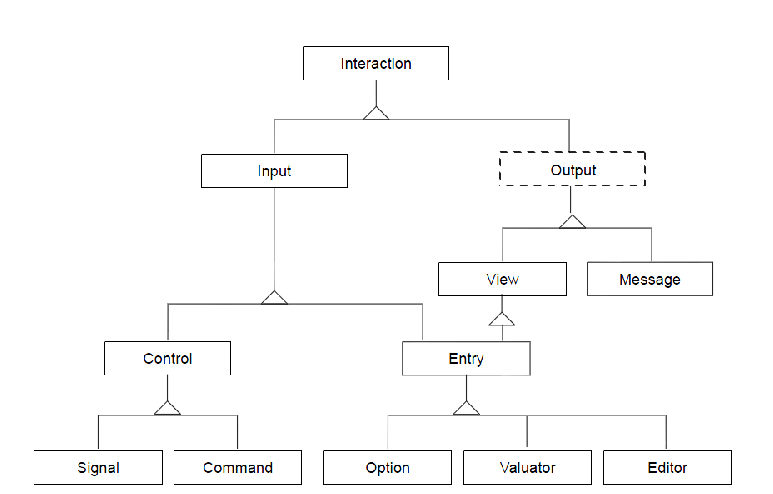
\includegraphics[width=353pt]{chap2/img-5.eps}
\caption{Modèle d'interactions abstraites de Gellersen}\label{fig:chap2:15}
\end{center}
\end{figure}


Dans le cadre du changement de modalité d'interaction entrainé par la migration, ce modèle permet de décrire les interactions des différents composants 
graphiques de l'UI de manière indépendante des modalités d'interactions. Par exemple une fenêtre d'authentification comportant des champs de texte et des boutons, les champs de texte seront représentés par les Editor qui sont des interactions à la fois en entrée et en sortie et les boutons seront représentés par des Command dans un modèle abstrait. 

Ce modèle identifie à la fois les interactions en entrée et en sortie de haut niveau et indépendamment des modalités d'interactions. Dans le cadre de la migration de l'UI CBA par exemple, les interactions telles que la rotation, le déplacement ou le redimensionnement qui sont liés aux guidelines de la table interactives doivent être interprétés comme des commandes. Cette interprétation n'est pas générique et dépend du concepteur des interactions,  en effet le déplacement peut être considéré comme une rotation en modifiant l'angle par exemple. De manière générale, le modèle de Gellersen est un modèle d'interactions abstraites qui nécéssite la spécification de certaines interactions indépendantes des modalités d'interactions pendant la migration.


\subsubsection{Résumé}
\fbox{\parbox{0.9\textwidth}{
Deux caractéristiques sont essentielles pour les modèles d'interactions abstraites : 
\begin{itemize}
\item leurs indépendances d'une modalité d'interaction 
\item et leur capacité à décrire toutes interactions du langage d'une modalité. 
 \end{itemize}
}}

\section{Conclusion}
\label{sec:chap2:6}
Dans ce chapitre nous avons étudié les problèmes liés à la migration d'UI vers une table interactive qui consiste à:
\begin{itemize}
\item transformer le layout de l'UI de départ conformément aux guidelines pour les UI collaboratives
\item changer les modalités d'interactions de l'application de départ conformément aux guidelines pour les UI tangibles et tactiles
\item adapter la taille et le style de l'UI de départ aux recommandations de la plateforme d'arrivée.
\end{itemize}

Dans le chapitre suivant, nous étudions quelques mécanismes de migration des UI en faisant ressortir les problématiques liées à la prise en compte des guidelines et au changement de modalités d'interactions de ces mécanismes de migration.